% !TeX root = ../smc-report.tex
% !TeX encoding = UTF-8
% !TeX spellcheck = en_GB

\section*{PRISM Tutorial Part 3: Dynamic power management}

  \subsection*{Dynamic power management}

    In this section will be described the modelisation through PRISM \cite{KNP11} of a \textit{DPM} (\textit{Dynamic Power Management}) system, following the PRISM tutorial found at \cite{prism-tutorial3}. DPMs are used to apply different power usages to some computing device, according to a predefined strategy that takes into account the current state of the device. This kind of systems have been studied largely in literature, for example in \cite{qiu2001stochastic} where a DPM for a Fujitsu disk drive has been studied.
    
    A generic DPM system is made of three distinct components:
    
    \begin{itemize}
      \item \textit{Service Queue} (\textit{SQ}): holds the requests that the Service Provider will have to serve, in an ordered fashion, and can have finite queue capacity;
      \item \textit{Service Provider} (\textit{SP}): serves, one at a time, the requests stored in the Service Queue, serving each time the request at the head of the queue;
      \item \textit{Power Manager} (\textit{PM}): can change the power state of the Service Provider according to certain policies.
    \end{itemize}
    
    The \textit{SP} could be anything that is a computing device that serves requests, such as a disk drive as in \cite{qiu2001stochastic}, but also a CPU or a Web Server.
    
    At any given time, the \textit{SP} is in one of three possible power states, each of which:
    
    \begin{itemize}
      \item \textit{sleep}: the \textit{SP} is in a low-power consumption mode and is unable to serve any request unless explicitly awaken by the \textit{PM};
      \item \textit{idle}: the \textit{SP} is awake but currently not serving any request, so any newly arriving request will be served immediately by the \textit{SP};
      \item \textit{busy}: the \textit{SP} is currently serving a request and will be available to serve the next in queue as soon as it's finished.
    \end{itemize}
    
    Ideally, when in the \textit{sleep} state the \textit{SP} will be requiring little to none power, when in the \textit{idle} state it will require more, as it is awake and ready to serve requests, while when \textit{busy} it will require even more, as the \textit{SP} in that case is actively working on a request. The \textit{PM} is charged with employing a power consumption strategy by switching the \textit{SP}'s power state, in order to maximise the availability of the service while minimising the overall power consumption.
    
    A first PRISM model for a DPM based on \cite{qiu2001stochastic} is proposed in Code \ref{lst:power}, as seen in \cite{prism-tutorial3}.
    
    \begin{center}
      \lstinputlisting[language=prism, caption={PRISM code for the model of a DPM based on \cite{qiu2001stochastic}, with only the \textit{SQ} and the \textit{SP} components. Source \cite{prism-tutorial3}.}, label={lst:power}]{code/power.sm}
    \end{center}
    
    In this first model version shown in Code \ref{lst:power}, only the two modules, for the \textit{SQ} and the \textit{SP} components, are introduced. This is an already working strategy, even without the \textit{PM} component, which would only add a smarter policy for the \textit{SP}'s power management.
    
    It is worth noticing that the model shown in Code \ref{lst:power} is described as a \textit{Continuous Time Markov Chain} (\textit{CTMC}), which allows the use of rates when defining the firing of transitions instead of simple probabilities.
    
    \question{Read the section on \href{http://www.prismmodelchecker.org/manual/ThePRISMLanguage/Synchronisation}{synchronisation} in the manual. Then, have a look at the definition of the \prism{SQ} and \prism{SP} modules, and try to understand what they describe.}
    \answer{
      The \prism{SQ} and \prism{SP} modules implement, respectively, the \textit{SQ} and \textit{SP} components of the DPM system. Both modules synchronise on three different kinds of actions: \prism{request}, indicating the arrival of a new request, \prism{serve}, indicating that a request (except the last) has been served, and \prism{serve_last}, indicating that the last request in the queue has been served.
      
      The \prism{SQ} module keeps a variable, \prism{q}, that represents the current number of request in the queue, with maximum capacity given by the constant \prism{q_max}. When, with the predefined arrival rate \prism{rate_arrive}, a new request arrives (line 26) the queue is updated accordingly, eventually discarding requests in excess in case of a full queue. When a request is served by the \prism{SP} module, whether it was the last (line 30) or not (line 28), the queue is decreased accordingly. The distinction for these two cases might seem useless on the \prism{SQ} side, but it will prove useful for the \prism{SP} module.
      
      The \prism{SP} module only keeps a variable, \prism{sp}, indicating the current power state (0 meaning \textit{sleep}, 1 \textit{idle} and 2 \textit{busy}), which starts in the \textit{idle} state. When a new request arrives, the \textit{SP} is switched to the \textit{busy} state in case it was \textit{idle} (line 51), indicating that it started working on that request right away, while if the power state is either \textit{sleep} or \textit{busy} then it's kept the same (line 54). When a request that was not the last in the queue is served (line 52), with service rate defined by the variable \prism{rate_serve}, the \textit{SP} is kept in the busy state, meaning that it starts working on the next request in line. Otherwise, if the last request is served (line 58), employing the same service rate, the \textit{SP} is switched back to the \textit{idle} state.
      
      It is worth noticing that, since by definition only the \textit{PM} component can decide when the \textit{SP} has to wake, in this first model, if the \textit{SP} starts in the \textit{sleep} state, it would have no way of awaking.
    }
    
    \question{Download the model file \bash{power.sm} from above and load it into PRISM.\\}
    \trivialanswer{
      The model \bash{power.sm} loaded into PRISM is shown in Figure \ref{fig:loaded_model}.
    	\begin{figure}[h!]
    		\begin{center}
    			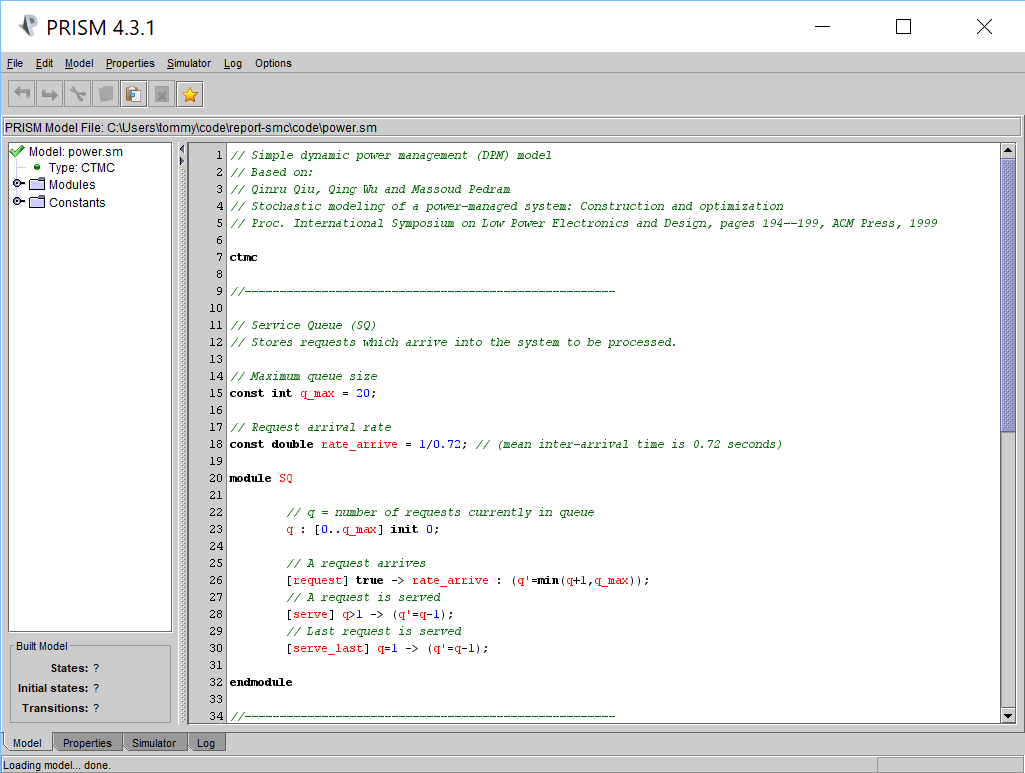
\includegraphics[scale=0.8]{loaded_model.png}
    		\end{center}
    		\caption{Model \bash{power.sm} loaded into PRISM.}
    		\label{fig:loaded_model}
    	\end{figure}
    }
    
    \question{Use the PRISM simulator to generate some random paths through the model. Notice how, for a CTMC model like this, the elapsed time as the path progresses is displayed in the table. You will probably find that the size of the queue (\prism{q}) never gets above 1. Why is this? Generate a path by hand where the queue reaches its maximum size (currently \prism{q_max}=20). What happens when more requests arrive while the queue is full?}
    \answer{
      By repeatedly selecting the ``Simulate'' button in the PRISM simulator with 1 step it can effectively be seen that the queue size almost never exceeds 1. This because of how arrival and service rates are defined: while the arrival rate of new requests is $1.3\overline{8}$, meaning that on average a new request arrives every $0.72$ seconds, the service rate is $125$, meaning that on average a request is served in $0.008$ seconds. This means that, when a request is in the queue, the service time of that request is, on average, $90$ times faster than the arrival of a new request. So, although possible, it's just highly unlikely that, with rates so defined, a new request arrives before a service is finished.
      
      If instead the action \prism{request} is repeatedly selected in the PRISM simulator in order to force the arrival of new requests before the service, a full queue can be reached. In this case, as expected, more request arrivals end up in the refusal of these new requests, simply no including them in the queue, which remains at it's full capacity (\prism{q_max}=20 in this case). It is worth noticing that, in case a new request arrives before a service is completed, even though the \prism{serve} action remains enabled, it's probability distribution remains the same, since these are all exponentially distributed transitions and thus memoryless.
    }
    
    \question{What is the size of the state space of this model? (i.e from the initial state, how many possible different states can be reached?) Go back to the ``Model'' tab of the GUI, select menu option ``Model | Build model'' and then look at the statistics displayed in the bottom left corner to check your answer.}
    \answer{
      By selecting the ``Build model'' feature, it can be seen that the state space of this model is made of a total of 21 states. Intuitively, these are made of a state where the \textit{SP} is \textit{idle} and the queue empty and 20 states where the \textit{SP} is \textit{busy} and the queue has a different number of pending requests (from 1 to 20).
    }
    
  \dashedrule
  
  \subsection*{Adding the power management control}
  
    Now we add to the PRISM model shown in Code \ref{lst:power} and additional module, \prism{PM}, responsible of implementing the Power Manager. The \textit{PM} is the component of a DPM that is charged with waking the \textit{SP} from sleep or putting it back to sleep according to a specific policy that might be dependent of several factors, such as the current state of the \textit{SP} or of the \textit{SQ}.
    
    Code \ref{lst:power_policy1} shows the updated model with the added \prism{PM} module, which employs a fairly naive policy.
    
    \begin{center}
      \lstinputlisting[language=prism, caption={PRISM code for the model of a DPM based on \cite{qiu2001stochastic}, with the \textit{SQ}, \textit{SP} and \textit{PM} components. Source \cite{prism-tutorial3}.}, label={lst:power_policy1}]{code/power_policy1.sm}
    \end{center}
    
    \question{Look at the code we have added to the \prism{SP} module and at the new \prism{PM} module. Make sure you understand how they work.}
    \answer{
      The \prism{PM} module has the function of wake the \textit{SP} or to put it back to sleep according, in this case, to the current size of the queue.
      
      In particular, when in the queue there are at least \prism{q_trigger} elements the modules \prism{PM} and  \prism{SP} can synchronise on the action \prism{sleep2idle} (lines 56, 57 and 87), effectively waking up the \textit{SP} in case it was still asleep, as the action name suggests. If, when the awakening is triggered, the queue \prism{q} is empty then the \textit{SP} is switched to the \textit{idle} state, otherwise it's switched directly to the \textit{busy} state, i.e. working on the request on top of the queue.
      
      Whenever, instead, the queue becomes empty, the \prism{PM} and \prism{SP} modules can synchronize on the \prism{idle2sleep} action (lines 59 and 90), effectively waking up the \textit{SP}.
      
      It is worth noticing how the operations of waking the \textit{SP} up and putting it back to sleep are not immediate but instead, when the corresponding conditions are met, are characterised by rates (\prism{rate_s2i} and \prism{rate_i2s}, respectively). Also, in this second version of the model, the \prism{SP}'s power state is now initialised as 0 (i.e. \textit{sleep} state), since now, thanks to the \prism{PM} module, initialising the \textit{SP} in the \textit{sleep} state wouldn't end up in a deadlock any more.
    }
    
    \question{Now use the simulator to generate a trace through this new model. When you create a new path, you have to specify a value for the constant \prism{q_trigger}, because it is left undefined in the model. Try a value of 5 for now. Does this new model behave as you expect?}
    \answer{
      After a few simulation steps, it can be seen that the model actually behaves as expected. In particular, between 0 and 4 requests the \textit{SP} has no other option than staying in the \textit{sleep} state and, thus, the model has just one available transition at each step, that is the arrival of new requests. When the queue reaches 5 requests, the waking condition is met, but sometimes the awakening is not immediate and some additional requests (usually 1 or 2) manage to arrive before the \textit{SP} is properly awaken: this is due the fact that the awaking rate (\prism{rate_s2i}) is slightly smaller than the request arrival rate (\prism{request}), meaning that on average the arrival of a new request is slightly faster than the awakening of \textit{SP}.
      
      Similarly, once the queue has been emptied, the \textit{SP} can be switched back to \textit{sleep} right away or it could happen that a request manages to arrive before that happens, forcing the \textit{SP} to serve it first by switching to the \textit{busy} state.
    }
    
  \dashedrule
    
  \subsection*{Analysing the model}
  
    We'll analyse now various aspects of the model, exploiting the properties and analyses features that PRISM offers.
    
    \question{
      Go to the "Properties" tab of the GUI, create a new constant called T, of type double and with no defined value. Then add the following property:
      
      \lstinputlisting[language=prism, numbers=none]{code/q_max_P.pctl}
    }
    \trivialanswer{
      The property regarding the full queue added through the PRISM interface is shown in Figure \ref{fig:q_max_property}.
      
    	\begin{figure}[h!]
    		\begin{center}
    			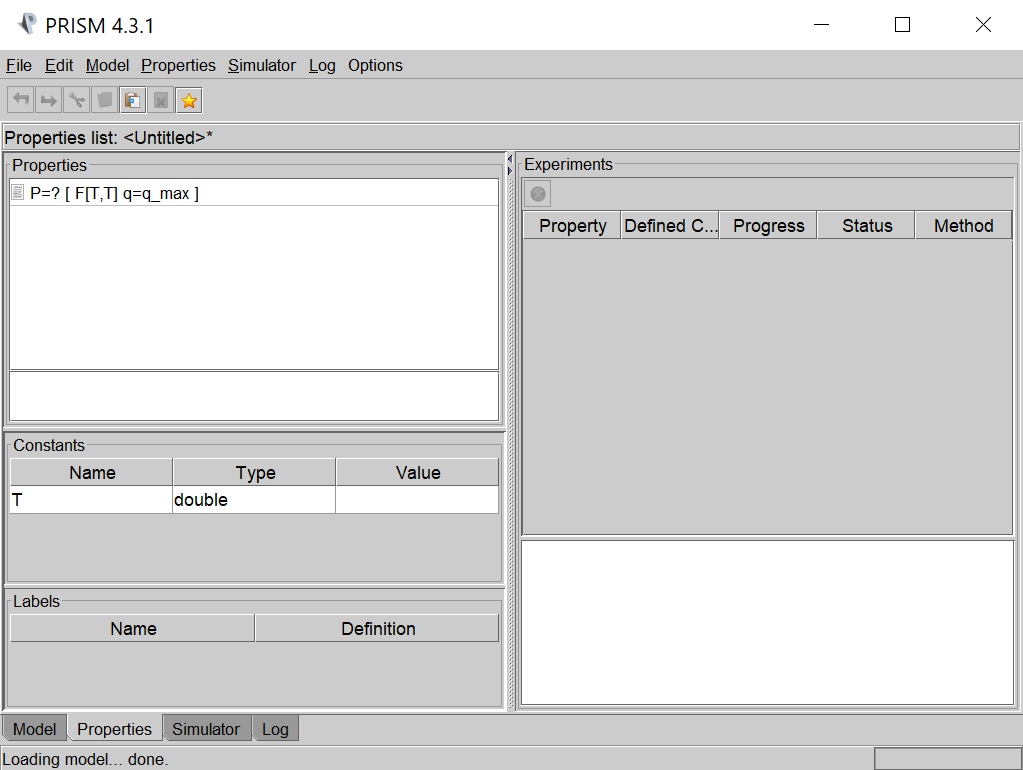
\includegraphics[scale=0.8]{q_max_property.png}
    		\end{center}
    		\caption{Full queue property added in PRISM.}
    		\label{fig:q_max_property}
    	\end{figure}
    }
    
    \question{Now, create an \href{http://www.prismmodelchecker.org/manual/RunningPRISM/Experiments}{experiment} based on this property, plotting a graph of its result for \prism{q_trigger} equal to 5 and \prism{T} from 0 up to 20, i.e. for the first 20 seconds of the system.}
    \answer{
      The resulting experiment plot, with steps of $0.5$ seconds, is shown in Figure \ref{fig:q_max_plot_0-20}.
    	\begin{figure}[h!]
    		\begin{center}
    			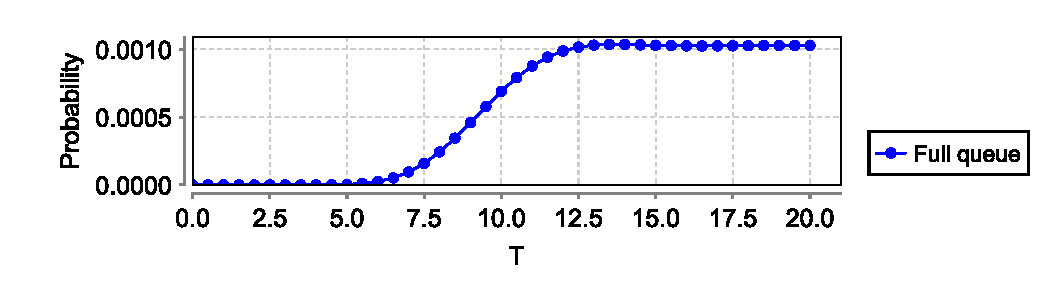
\includegraphics[scale=0.45]{q_max_plot_0-20.eps}
    		\end{center}
    		\caption{Experiment plot of the full queue between time 0 and 20.}
    		\label{fig:q_max_plot_0-20}
    	\end{figure}
    }
    
    \question{It seems that the transient probability of the queue being full stabilises after a short while. Using another experiment, plot values for the same property on the same graph, this time for \prism{T} from 20 up to 40, and see if the probability remains the same. To confirm this, now create a property to check the long-run probability of the queue being full, using the \href{http://www.prismmodelchecker.org/manual/PropertySpecification/TheSOperator}{S operator}. Right click the new property and select ``Verify''. You will need to give a value for \prism{T} but this is not used so you can enter anything. It turns out that the default iterative method in PRISM (Jacobi) for solving this kind of property does not converge in this case. Switch to the Gauss-Seidel method from the ``Options'' dialog and try again. Check that your result matches the graph.}
    \answer{
      From the extended plot shown in Figure \ref{fig:q_max_plot_0-40} it seems that the probability of reaching a full queue indeed stabilises.
      
    	\begin{figure}[h!]
    		\begin{center}
    			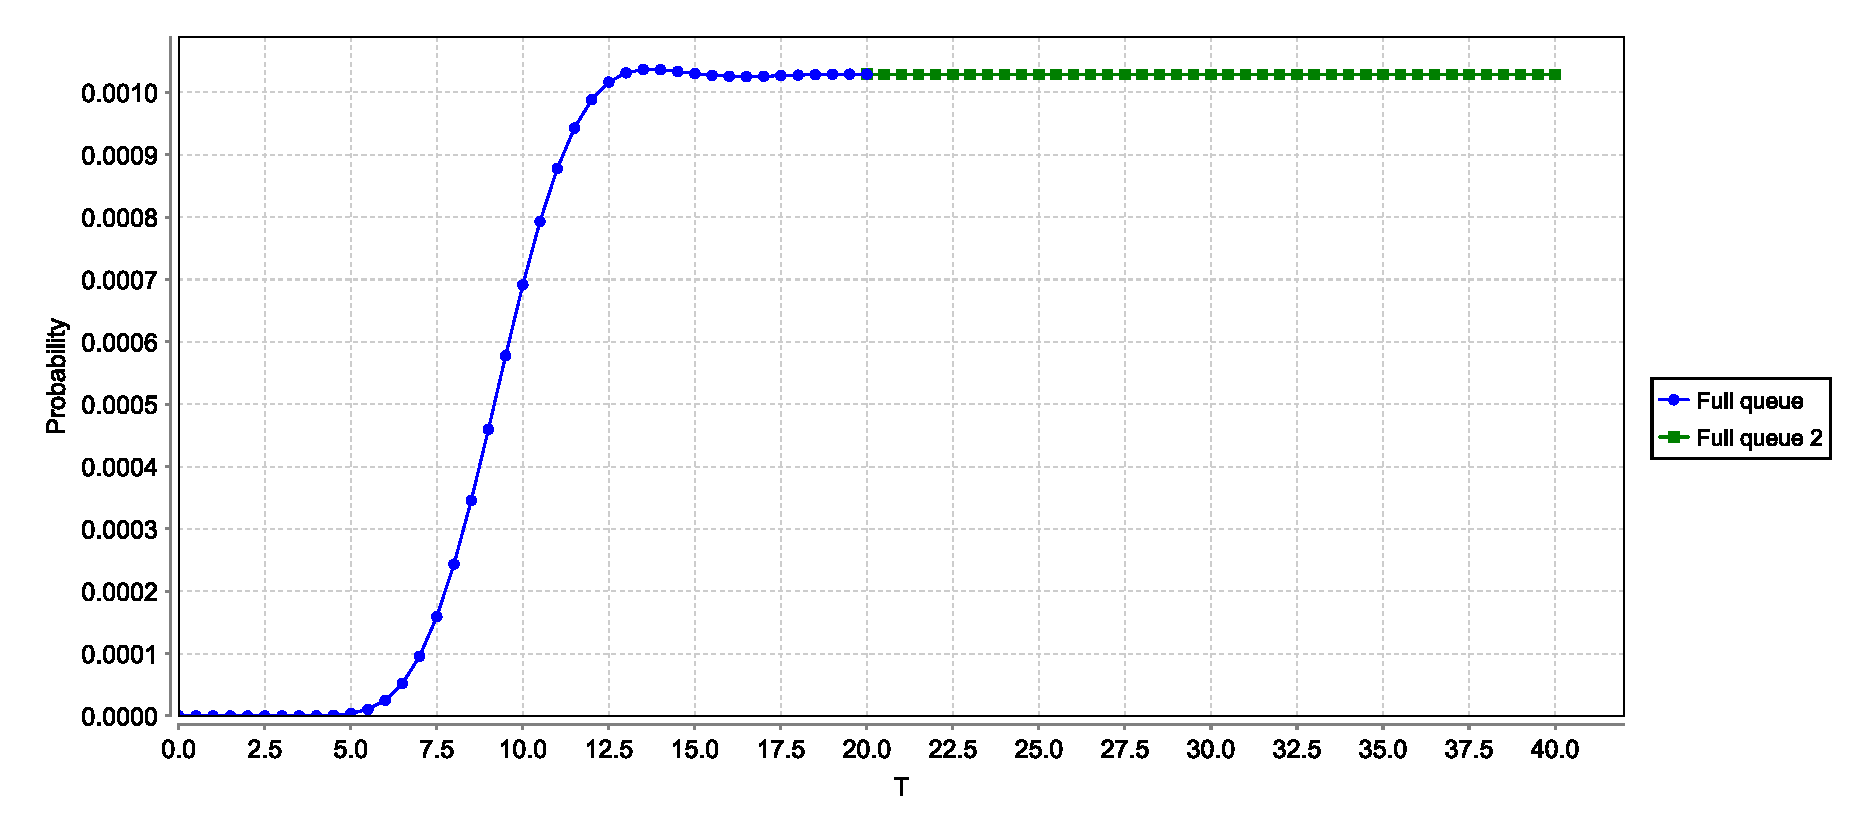
\includegraphics[scale=0.45]{q_max_plot_0-40.eps}
    		\end{center}
    		\caption{Experiment plot of the full queue between time 0 and 40.}
    		\label{fig:q_max_plot_0-40}
    	\end{figure}
    	
    	In order to check the steady-state probability of the queue being full in a more direct fashion, the following property, that exploits the S operator, can be used:
    	
      \lstinputlisting[language=prism, numbers=none]{code/q_max_S.pctl}
      
      By trying to evaluate the property using the default iterative method (Jacobi) the evaluation indeed does not converge and PRISM prompts an error. Instead, using the Gauss-Seidel iterative method, the computed steady-state probability of the queue being full results being $0.0010287642322871614$. Watching at the plot in Figure \ref{fig:q_max_plot_0-40} it looks like the probability of a full queue stabilises slightly above $0.0010$, which matches with the obtained result.
    }
    
    \question{Read the section on \href{http://www.prismmodelchecker.org/manual/ThePRISMLanguage/CostsAndRewards}{costs and rewards} in the manual. Then, look at the rewards that have already been defined in this model.}
    \answer{
      The only reward that has been defined in the model in Code \ref{lst:power_policy1} is \prism{queue_size} which, at any given time, is equivalent to the current number of requests present in the queue.
    }
    
    \question{
      Add these two properties which can be used to compute the transient and long-run expected queue size, respectively:
      
      \lstinputlisting[language=prism, numbers=none]{code/queue_size.pctl}
    }
    \trivialanswer{
      The properties regarding the queue size added through the PRISM interface are shown in Figure \ref{fig:queue_size_properties}.
      
    	\begin{figure}[h!]
    		\begin{center}
    			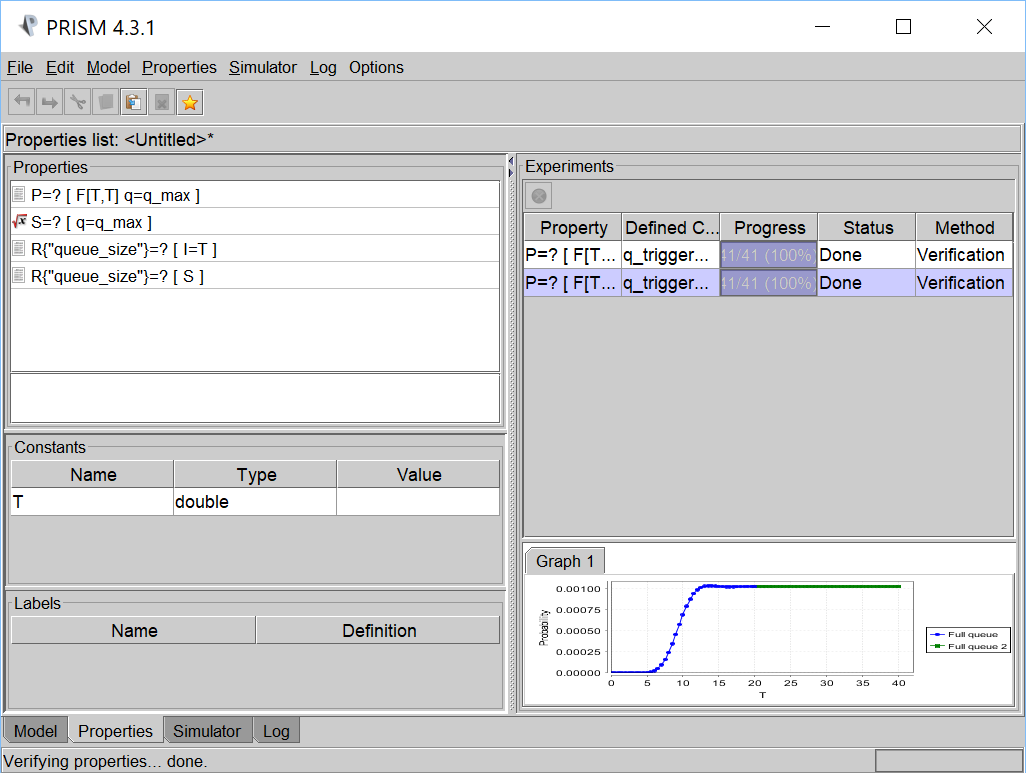
\includegraphics[scale=0.8]{queue_size_properties.png}
    		\end{center}
    		\caption{Queue size properties added in PRISM.}
    		\label{fig:queue_size_properties}
    	\end{figure}
    }
    
    \question{Plot the expected queue size at time \prism{T}, for the first 20 seconds of the model. As above, also compute the long-run value and check that it matches the results on the graph.}
    \answer{
      The experiment plot is shown in Figure \ref{fig:queue_size_plot}.
      
    	\begin{figure}[h!]
    		\begin{center}
    			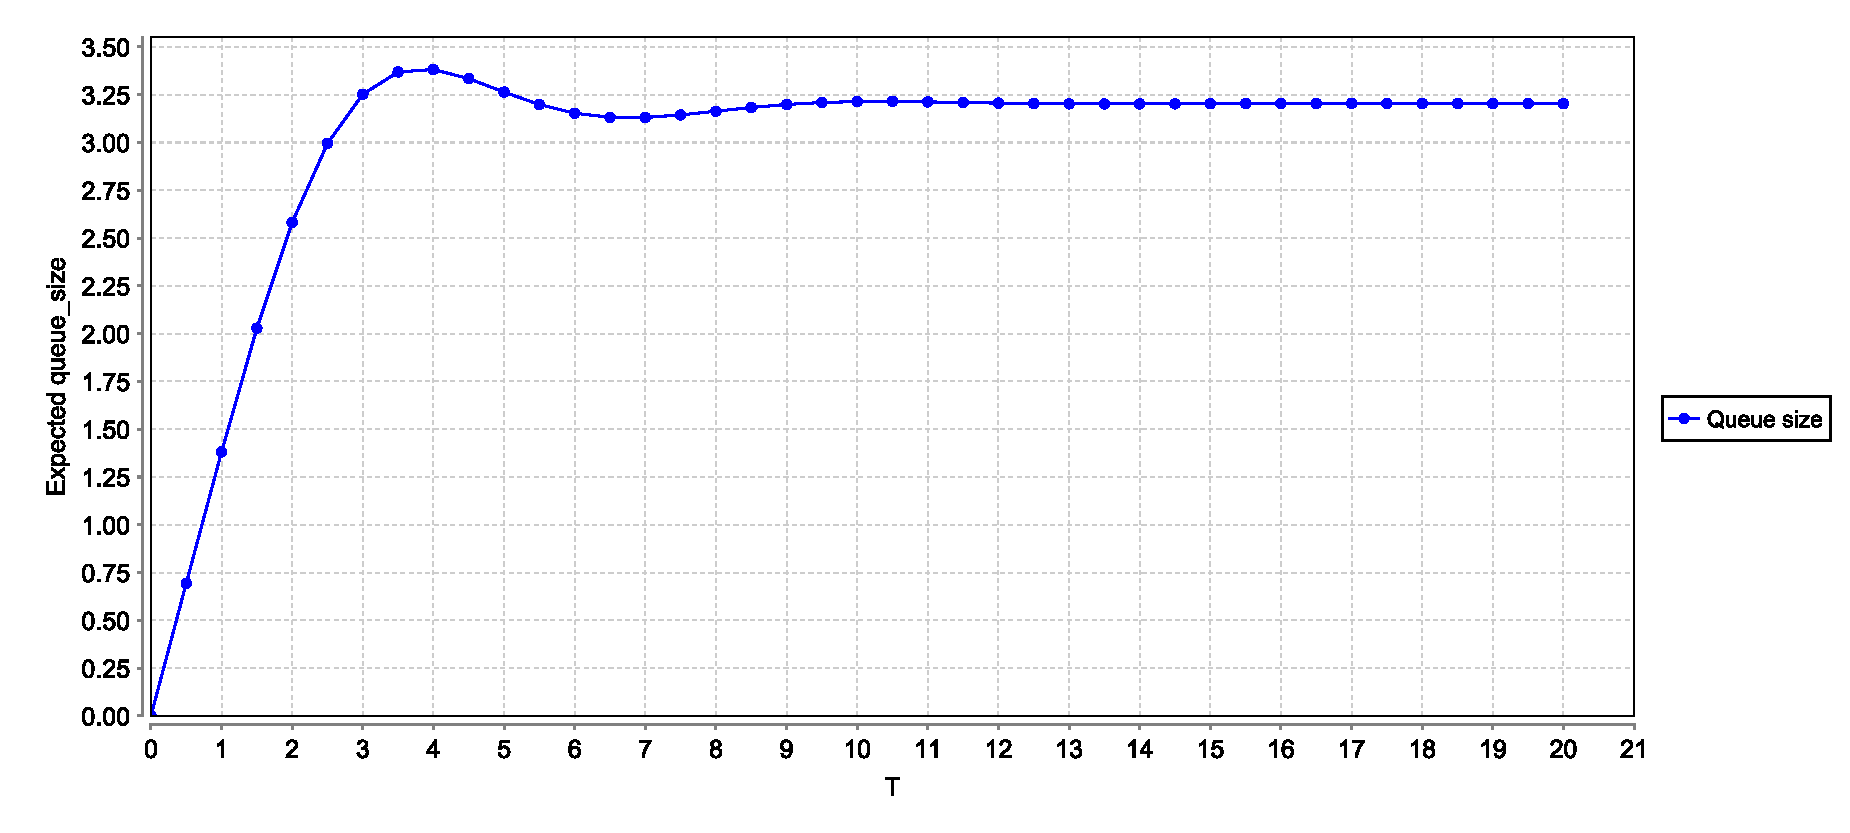
\includegraphics[scale=0.45]{queue_size_plot.eps}
    		\end{center}
    		\caption{Experiment plot of the queue size between time 0 and 20.}
    		\label{fig:queue_size_plot}
    	\end{figure}
    	
    	Evaluating instead the steady-state property, it can be seen that the number of requests in the queue at steady-state is $3.2038846166301242$, which seems to match to the transient results shown in the plot in Figure \ref{fig:queue_size_plot}.
    }
    
    \question{Now create some experiments to analyse the transient and/or long-run expected queue size for a range of different values of the constant \prism{q_trigger}. How does the performance of the system vary as this changes? What is the ``best'' value of \prism{q_trigger}?}
    \answer{
      Transient analysis results between time 0 and 40 and for \prism{q_trigger} between 0 and 21 are shown in Figure \ref{fig:queue_size-q_trigger_plot_I}. The last value, \prism{q_trigger}=21, has been included to show what happens in a scenario where the \textit{SP} never wakes.
      
    	\begin{figure}[h!]
    		\begin{center}
    			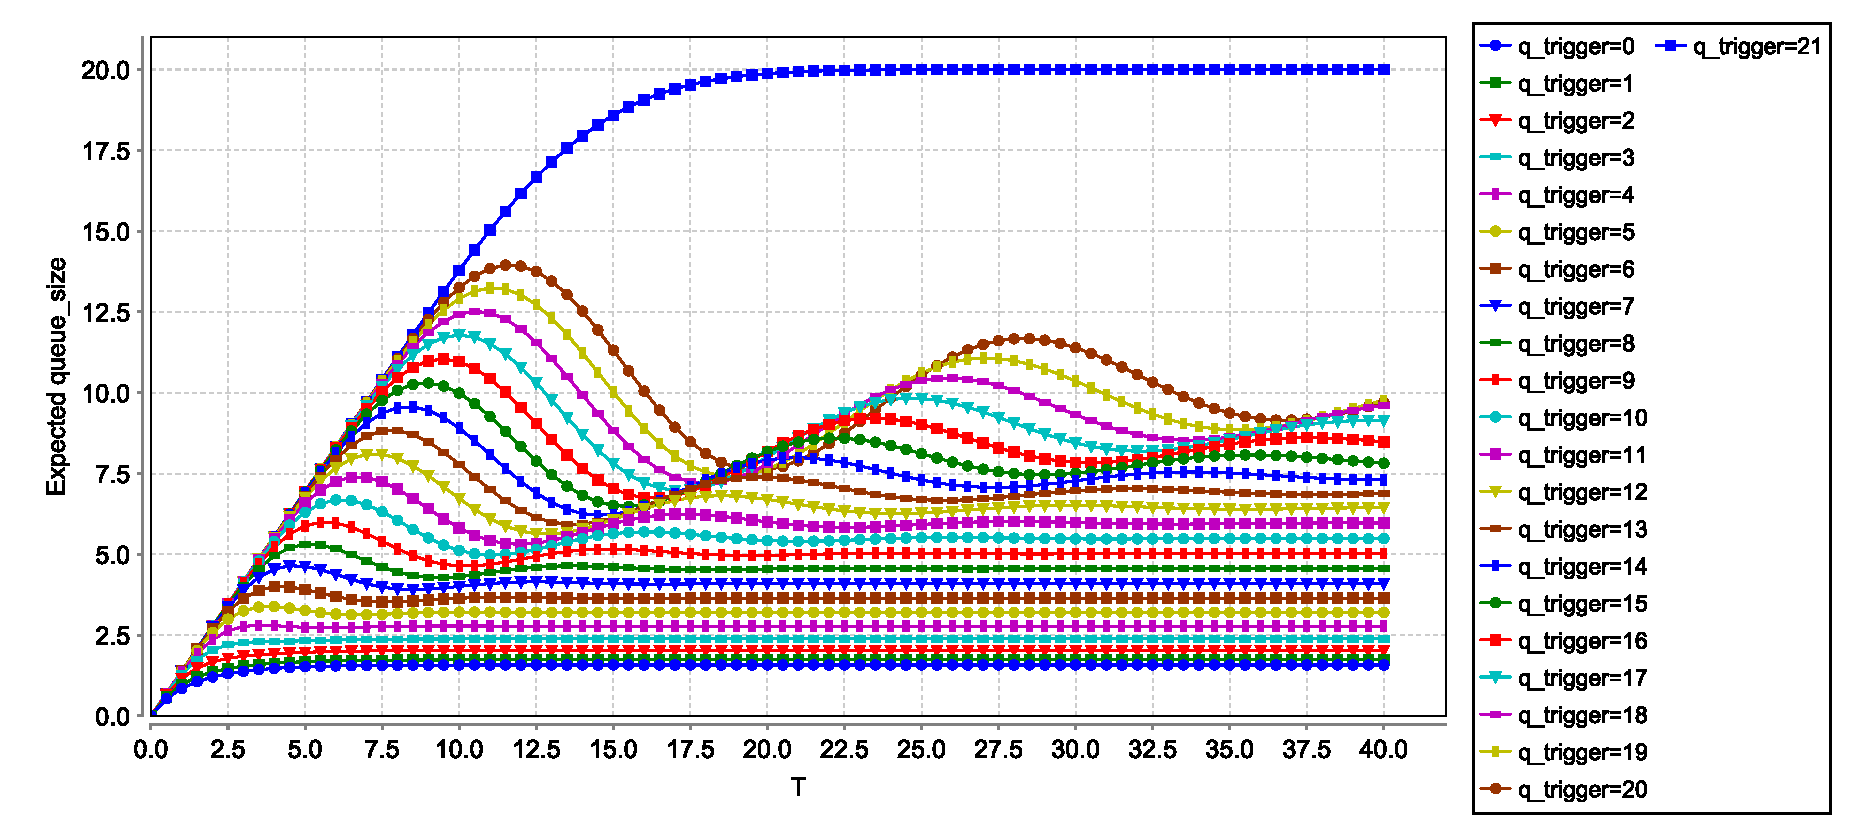
\includegraphics[scale=0.45]{queue_size-q_trigger_plot_I.eps}
    		\end{center}
    		\caption{Experiment plot of the queue size between time 0 and 40 and for \prism{q\_trigger} between 0 and 21.}
    		\label{fig:queue_size-q_trigger_plot_I}
    	\end{figure}
      
      As expected, the average queue size is higher for higher values of \prism{q_trigger}. After some time this value tends to stabilise, although for higher values of \prism{q_trigger} it seems as it needs more time in order to reach the steady-state. For \prism{q_trigger}=21, as expected, the queue fills completely and never gets the change to get emptied. According to the plot in Figure \ref{fig:queue_size-q_trigger_plot_I} we could say that the ``best'' values for \prism{q_trigger} are the lowest (from 0 to 5), since for those values the average queue size stabilises earlier, thus producing a more predictable behaviour.
      
      In Figure \ref{fig:queue_size-q_trigger_plot_S} is instead shown the average queue size at steady-state, for the same range of values for \prism{q_trigger}.
      
    	\begin{figure}[h!]
    		\begin{center}
    			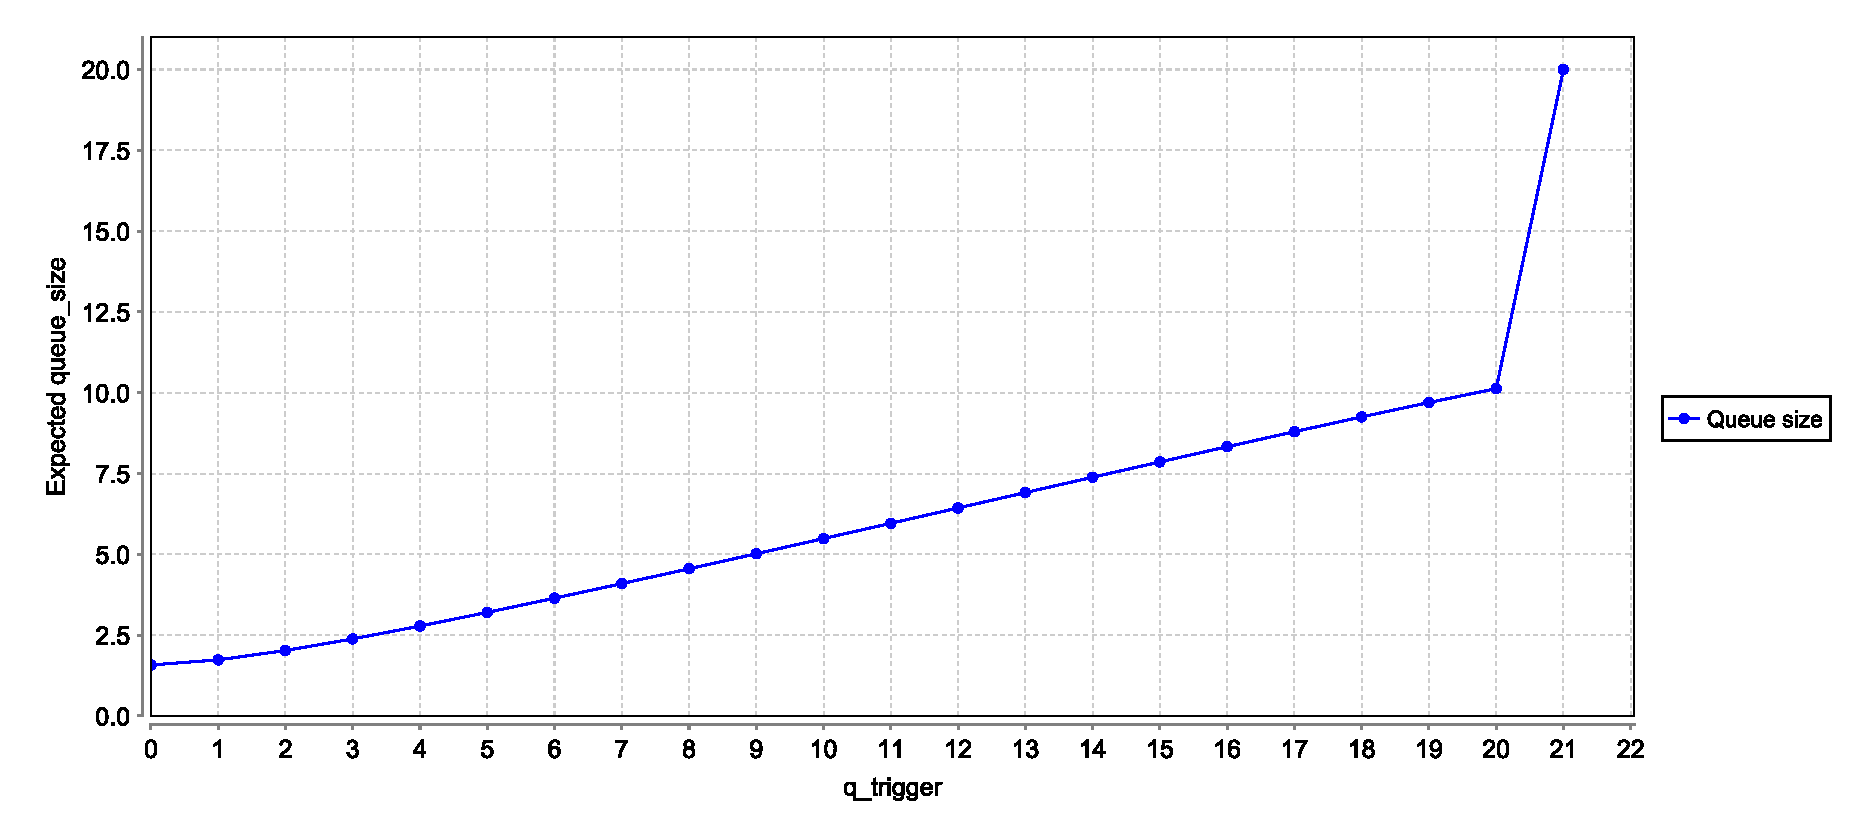
\includegraphics[scale=0.45]{queue_size-q_trigger_plot_S.eps}
    		\end{center}
    		\caption{Experiment plot of the queue size at steady-state for \prism{q\_trigger} between 0 and 21.}
    		\label{fig:queue_size-q_trigger_plot_S}
    	\end{figure}
      
      As expected, the average queue size rises as \prism{q_trigger} grows and it's exactly 20 for \prism{q_trigger}$\geq 21$. But is can also be observed that the growth is not exactly linear: for example for \prism{q_trigger}=1 the average queue size is $1.734$, while for \prism{q_trigger}=3 it's $2.383$.
      
      Ideally, we would like to have the queue as empty as possible at any time, because that would mean that requests are handled rapidly and there is more room for future requests, while at the same time consuming as few resources as possible, for example by keeping the \textit{SP} in the \textit{sleep} state for longer. In Figure \ref{fig:queue_size_coefficient_plot} we are showing then the \textit{queue size coefficient}, evaluated as \prism{q/q_trigger}, in order to find the best trade-off between these two factors. In particular, the coefficient is added to the PRISM model by including the following reward structure:
      
      \lstinputlisting[language=prism, numbers=none]{code/queue_size_coefficient.sm}
      
    	\begin{figure}[h!]
    		\begin{center}
    			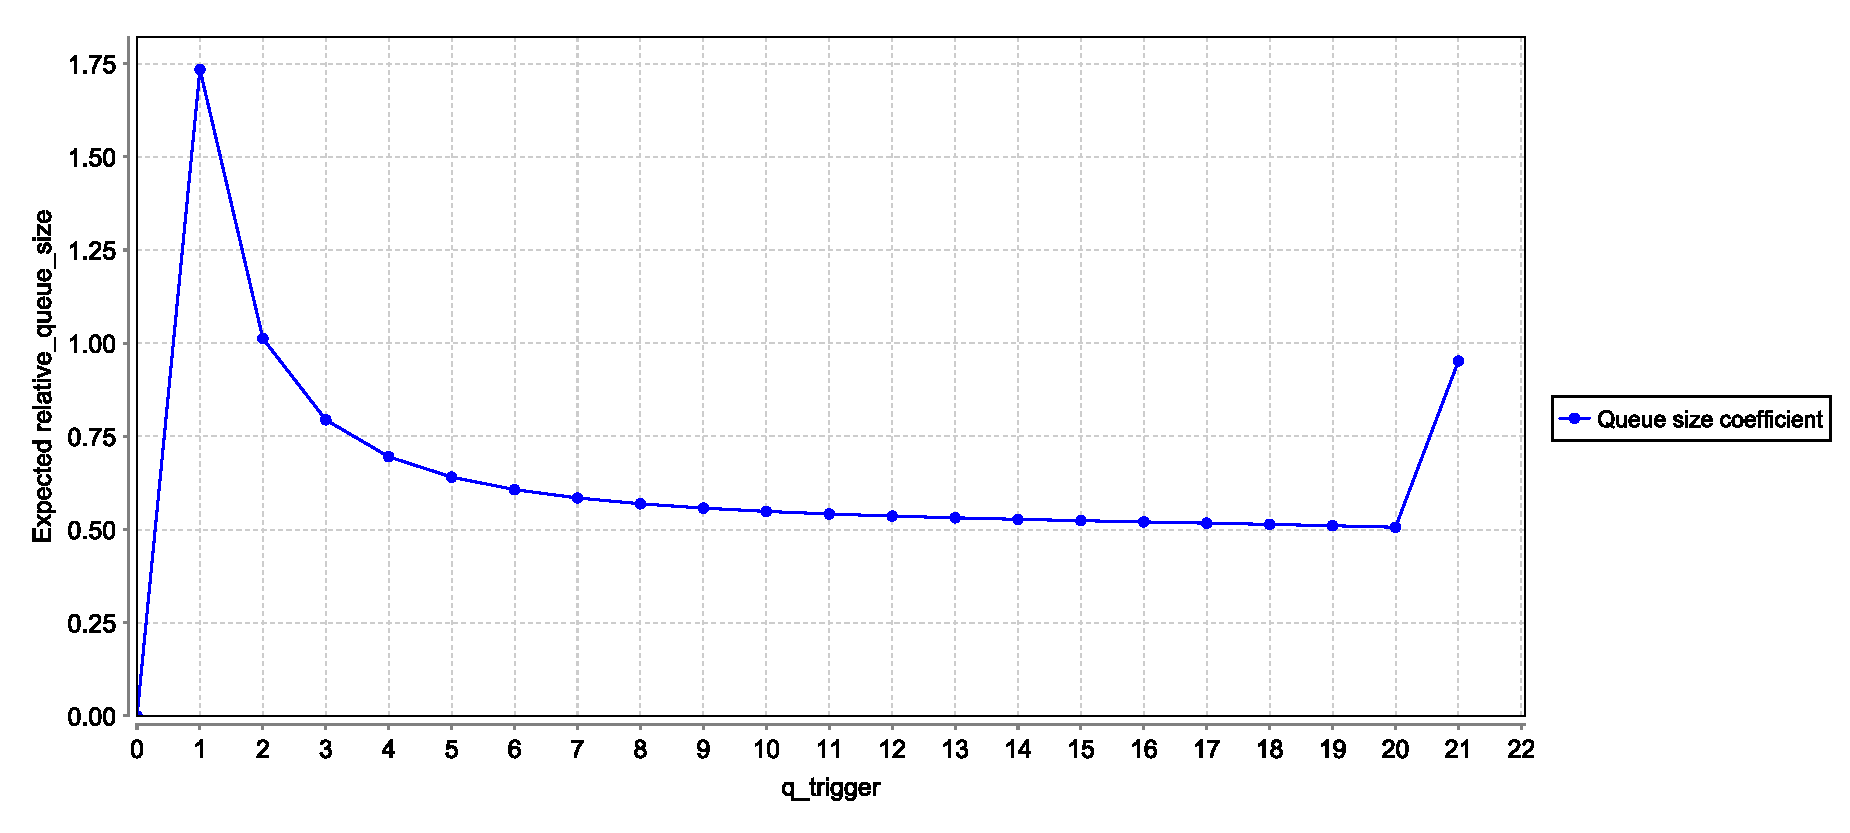
\includegraphics[scale=0.45]{queue_size_coefficient_plot.eps}
    		\end{center}
    		\caption{Experiment plot of the queue size coefficient at steady-state for \prism{q\_trigger} between 0 and 21.}
    		\label{fig:queue_size_coefficient_plot}
    	\end{figure}
      
      The results in Figure \ref{fig:queue_size_coefficient_plot} shows that, for \prism{q_trigger}=1 and 2, the coefficient is above 1, meaning that the average queue size is usually higher than the value of \prism{q_trigger}. For \prism{q_trigger}$\geq 3$ instead, the coefficient is lower than zero and decreasing, except for \prism{q_trigger}=21, which becomes higher again. According to this experiment then, we are able to say that the ``best'' value for \prism{q_trigger} is $20$, since in this case the queue size coefficient is at it's lowest (looking at the plot in Figure \ref{fig:queue_size-q_trigger_plot_S} we can see that for \prism{q_trigger}=20 the average queue size is $10.126$).
    }
    
    \question{Add a second \href{http://www.prismmodelchecker.org/manual/ThePRISMLanguage/CostsAndRewards}{reward structure} to the model called ``lost'', which assigns 1 to every transition of the model labelled with action \prism{request} from a state where the queue is full.}
    \answer{
      The reward ``lost'' is simply included in the PRISM model by adding at the end the following lines:
      
      \lstinputlisting[language=prism, numbers=none]{code/lost.sm}
    }
    
    \question{Now create a new property to check the expected \textit{cumulated} reward up until time \prism{T}. Don't forget to specify which reward structure you want in the property. (You might want to look at \href{http://www.prismmodelchecker.org/manual/PropertySpecification/Reward-basedProperties}{this section} of the manual.) How does this measure vary for different values of \prism{q_trigger}?}
    \answer{
      In Figure \ref{fig:lost_plot} are shown the results for the cumulative lost requests between time 0 and 40 and for values of \prism{q_trigger} between 0 and 20. The experiment is conducted using the following property:
      
      \lstinputlisting[language=prism, numbers=none]{code/lost_cumulative.pctl}
      
    	\begin{figure}[h!]
    		\begin{center}
    			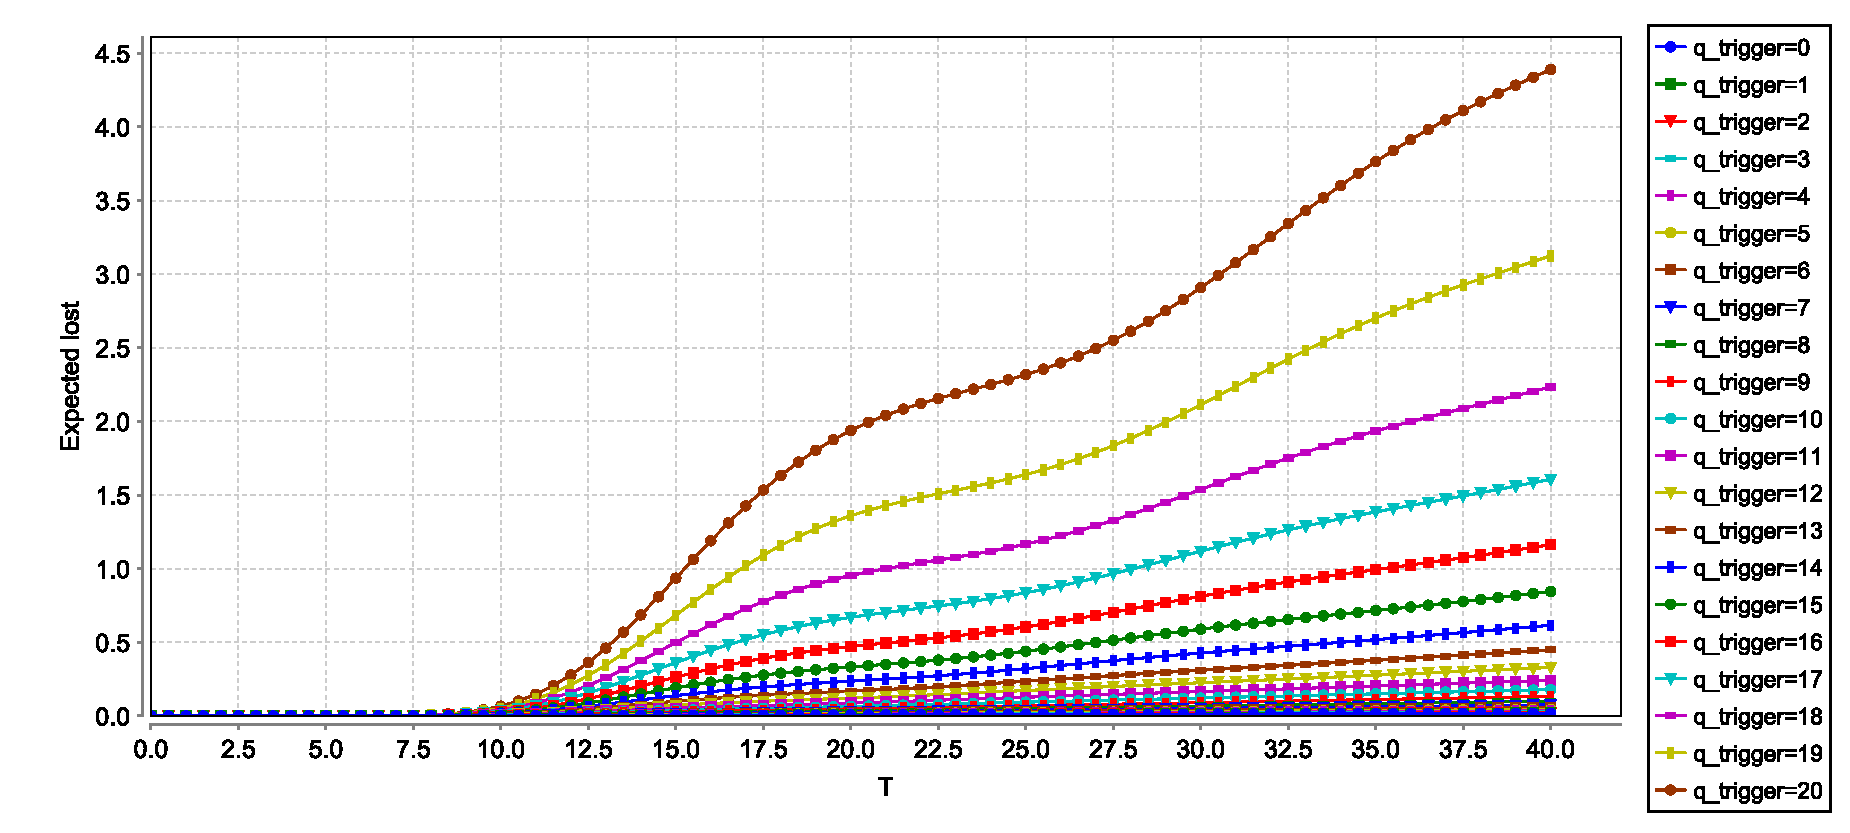
\includegraphics[scale=0.45]{lost_plot.eps}
    		\end{center}
    		\caption{Experiment plot of the cumulative lost requests between time 0 and 40 and for \prism{q\_trigger} between 0 and 20.}
    		\label{fig:lost_plot}
    	\end{figure}
      
      As expected, the cumulative lost requests are more as time goes on, but also for higher values of \prism{q_trigger} this values grows at higher rates. This is intuitive since when the \textit{SP} only wakes up after more requests have arrived in the queue, the chances of reaching the queue saturation are higher.
    }
    
    Let's imagine now to introduce a measure of the actual power consumption. In particular, energy consumption rates are $0.13$, $0.95$ and $2.15$, for the power states \textit{sleep}, \textit{idle} and \textit{busy}, respectively. On top of that, switching from \textit{sleep} to \textit{idle} costs $7.0$ energy units, while from \textit{idle} to \textit{sleep} costs $0.067$ energy units.
    
    \question{Add a third reward structure to the model representing the power consumption. Use a cumulative reward property to investigate the energy consumption over time of the system.}
    \answer{
      First of all, in order to add the desired reward structure, the following rates have to be included in the model:
      
      \lstinputlisting[language=prism, numbers=none]{code/consumption_rates.sm}
      
      Then, inside the \prism{SP} module, the following transitions have to be included:
      
      \lstinputlisting[language=prism, numbers=none]{code/consumption_transitions.sm}
      
      Finally, the ``consumption'' reward structure can be defined as follows:
      
      \lstinputlisting[language=prism, numbers=none]{code/consumption_reward.sm}
      
      Experiment results are shown in Figure \ref{fig:consumption_policy1_plot}.
      
    	\begin{figure}[h!]
    		\begin{center}
    			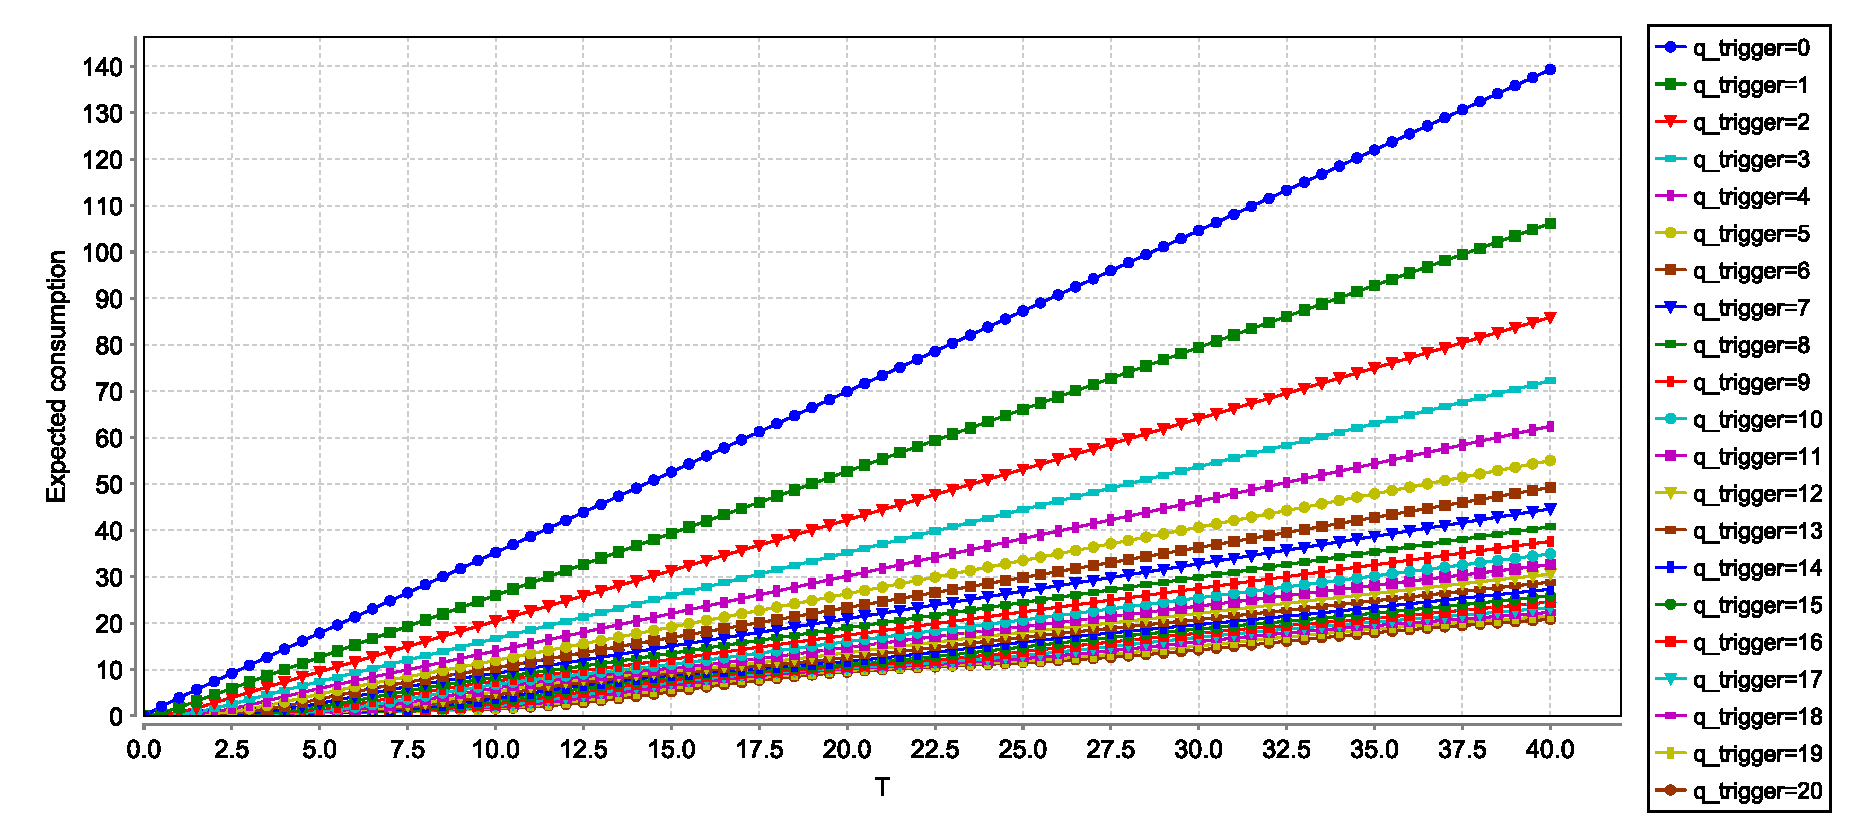
\includegraphics[scale=0.45]{consumption_policy1_plot.eps}
    		\end{center}
    		\caption{Experiment plot of the cumulative energy consumption between time 0 and 40 and for \prism{q\_trigger} between 0 and 20.}
    		\label{fig:consumption_policy1_plot}
    	\end{figure}
      
      As expected, the cumulative energy consumption grows as time goes on, but it can also be observed that the energy consumption is lower for higher values of \prism{q_trigger}, which is obvious considering that in these scenarios the \textit{SP} spends, on average, more time in the \textit{sleep} state, consuming less energy.
    }
    
  \dashedrule
  
  \subsection*{Extensions}
  
    \question{
      Replace the PM module in the existing model with the following:\\
      
      \lstinputlisting[language=prism, numbers=none]{code/PM_stochastic_policy.sm}
    }
    \trivialanswer{
      The model with stochastic policy loaded into PRISM is shown in Figure \ref{fig:loaded_model_stochastic_policy}.
    	\begin{figure}[h!]
    		\begin{center}
    			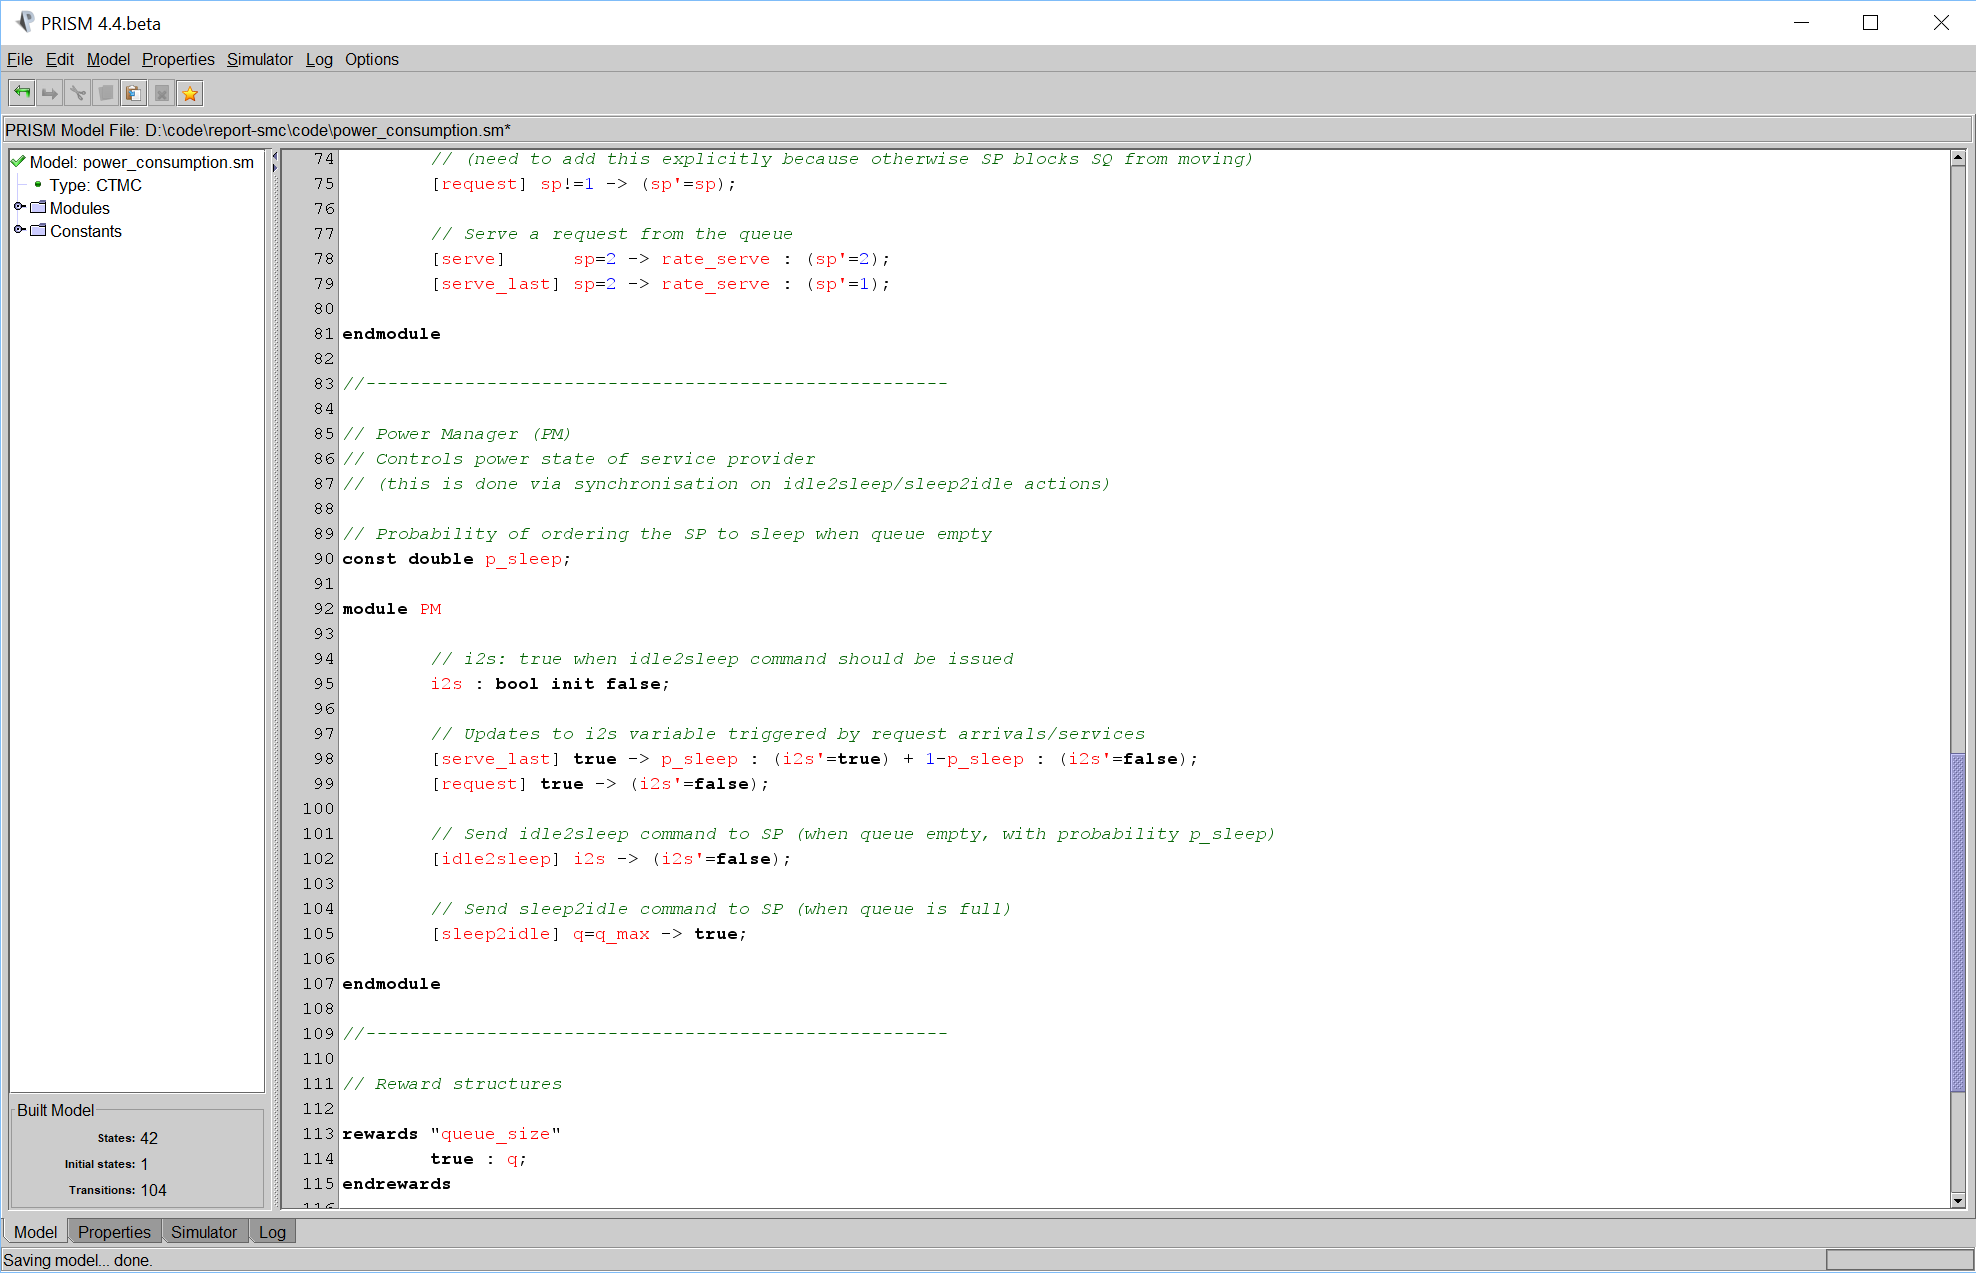
\includegraphics[scale=0.35]{loaded_model_stochastic_policy.png}
    		\end{center}
    		\caption{Model with stochastic policy loaded into PRISM.}
    		\label{fig:loaded_model_stochastic_policy}
    	\end{figure}
    }
    
    \question{How well does this power management system perform? What effect does the value of the probability \prism{p_sleep} have?}
    \answer{
      The results of the experiments concerning the cumulative energy consumption with the stochastic policy are shown in Figure \ref{fig:consumption_stochastic_plot}.
      
    	\begin{figure}[h!]
    		\begin{center}
    			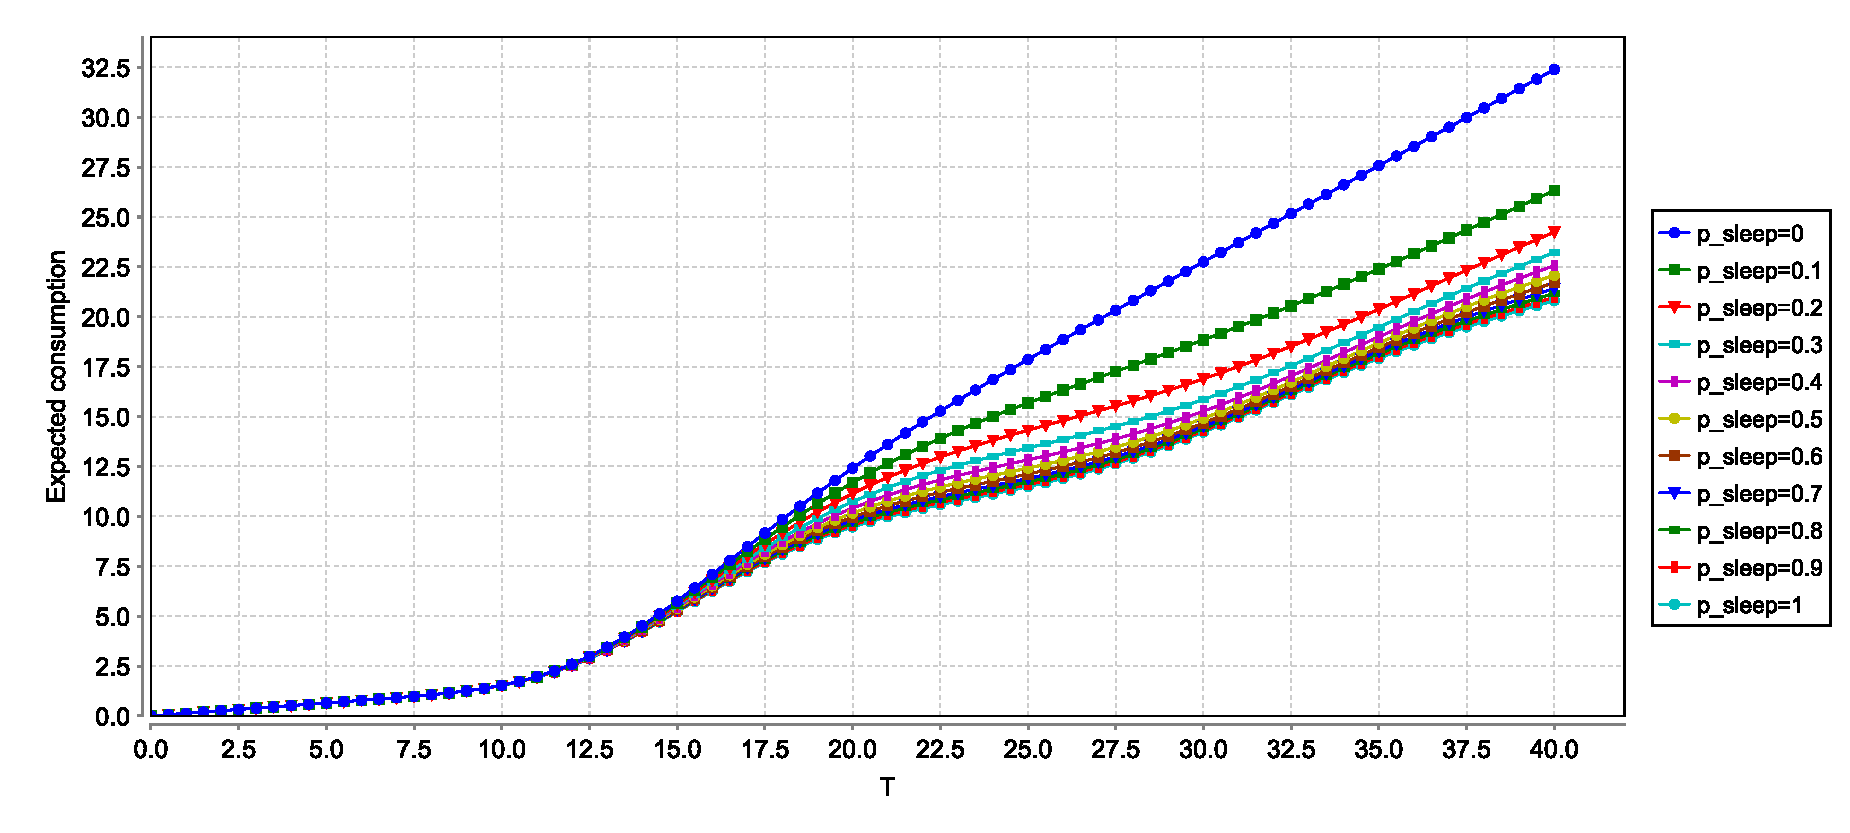
\includegraphics[scale=0.45]{consumption_stochastic_plot.eps}
    		\end{center}
    		\caption{Experiment plot of the cumulative energy consumption employing the stochastic policy, between time 0 and 40 and for \prism{p\_sleep} between 0 and 1, with step $0.1$.}
    		\label{fig:consumption_stochastic_plot}
    	\end{figure}
      
      Again, the energy consumption grows as the time goes on, but also it tends to be lower for higher values of \prism{p_sleep}, yielding top performance when \prism{p_sleep}=1, i.e. when the \textit{SP} always gets put to sleep after the queue has been emptied. On top of that, we can notice that while for the previous simpler policy the energy consumption, after 40 seconds, could reach, on average, almost 140 units (see Figure \ref{fig:consumption_policy1_plot}), with this new policy the maximum at \prism{T}=40 is $32.392$, for \prism{p_sleep}=0, making this second policy way more performing than the previous one.
    }
    
    \question{Can you think of any ways of improving these power management strategies? Implement them in the PRISM model and see how well they perform.}
    \answer{
      A possible way of minimising even further the energy consumption is to reverse the idea behind the stochastic policy introduced previously. In particular, we now want to always put the \textit{SP} to sleep when the queue has been emptied and wake it up only when the queue is full but only with a certain probability. This policy is implemented by the following code for the \prism{PM} module:
      
      \lstinputlisting[language=prism, numbers=none]{code/PM_custom_policy.sm}
      
      The results of the experimentation with this new policy are shown in Figure \ref{fig:consumption_custom_plot}.
      
    	\begin{figure}[h!]
    		\begin{center}
    			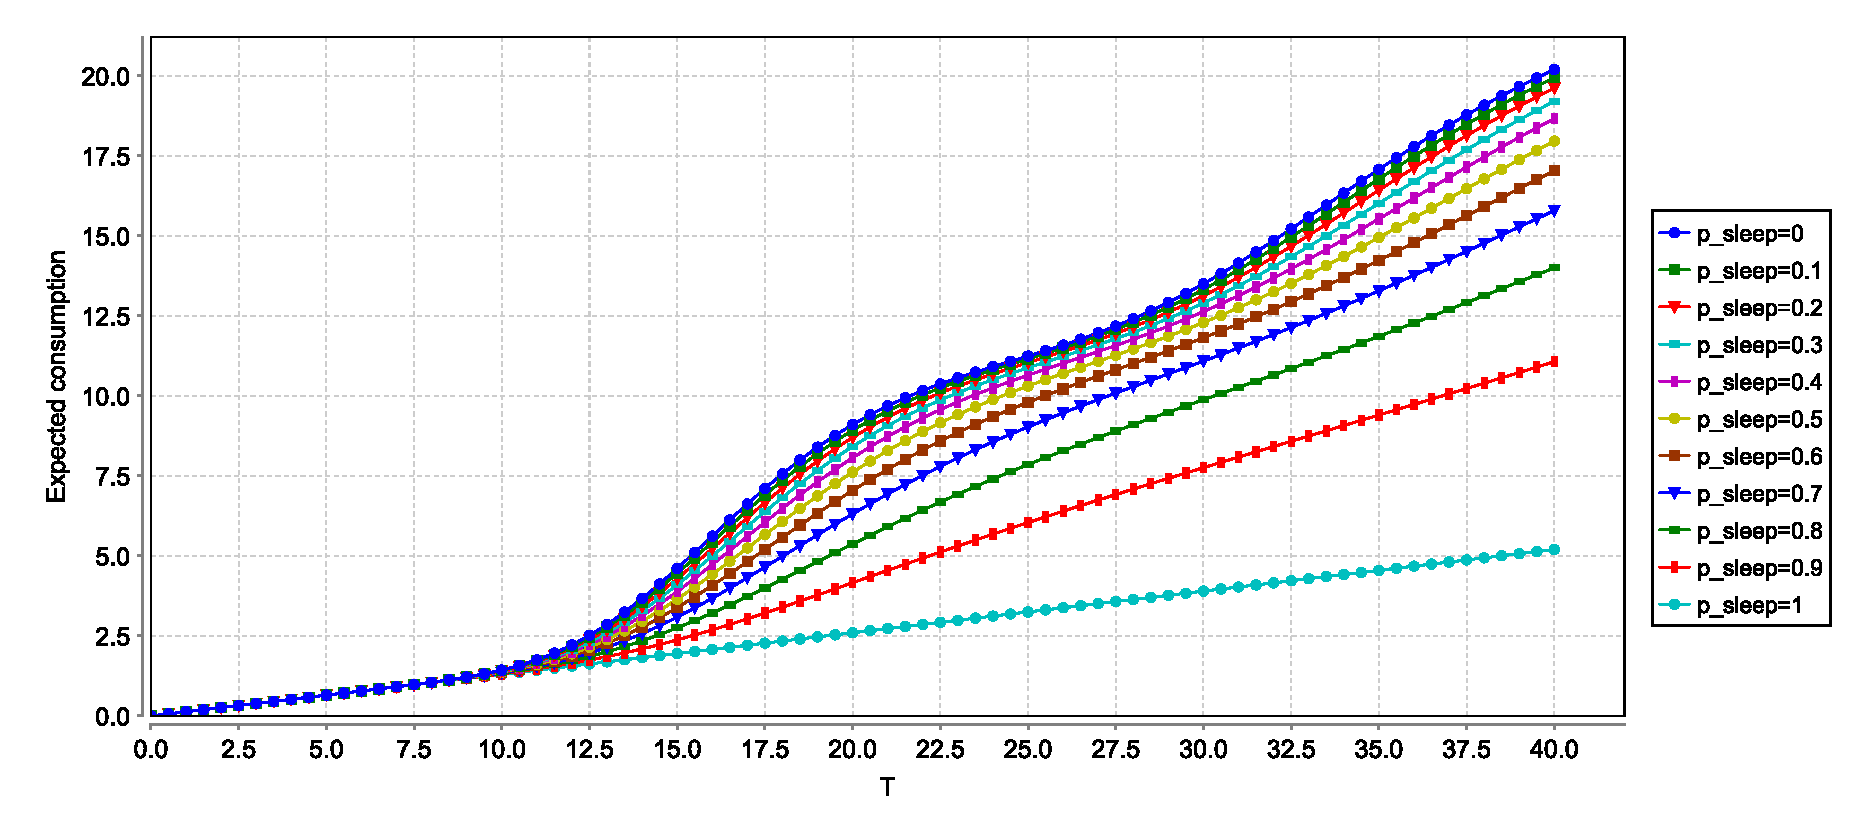
\includegraphics[scale=0.45]{consumption_custom_plot.eps}
    		\end{center}
    		\caption{Experiment plot of the cumulative energy consumption employing a new custom policy, between time 0 and 40 and for \prism{p\_sleep} between 0 and 1.}
    		\label{fig:consumption_custom_plot}
    	\end{figure}
      
      It can be observed that, by increasing the value of \prism{p_sleep}, i.e. the probability of remaining asleep even with a full queue, the cumulated energy consumption tends to be lower. This policy basically tries to minimise the number of times the \textit{SP} wakes up, being the wake up process a highly consuming action. Clearly, with this policy the number of lost requests is expected to be higher, but in a scenario where energy consumption is a central problem and some lost request is not such a big deal, this might be a good solution. In particular, the ``best'' case would be that with \prism{p_sleep}=1, but that would mean that the \textit{SP} never wakes up, which would be unrealistic.
      
      In order to further analyse the model, and devise smarter policies, both the energy consumption and the number of lost requests should be taken into account, in order to find the best trade-off.
    }
    
  \dashedrule
